
\dokumententypName{Checkup}

\RequirePackage{multirow}

% \schule@dokumentTypBezeichnung
\newcommand{\CheckupTitel}{{\usekomafont{title}Checkup \Titel: \usekomafont{reihe}\Reihe}} %\Linie
\newcommand{\CheckupBild}{%
	\begin{wrapfigure}{R}{2cm}
	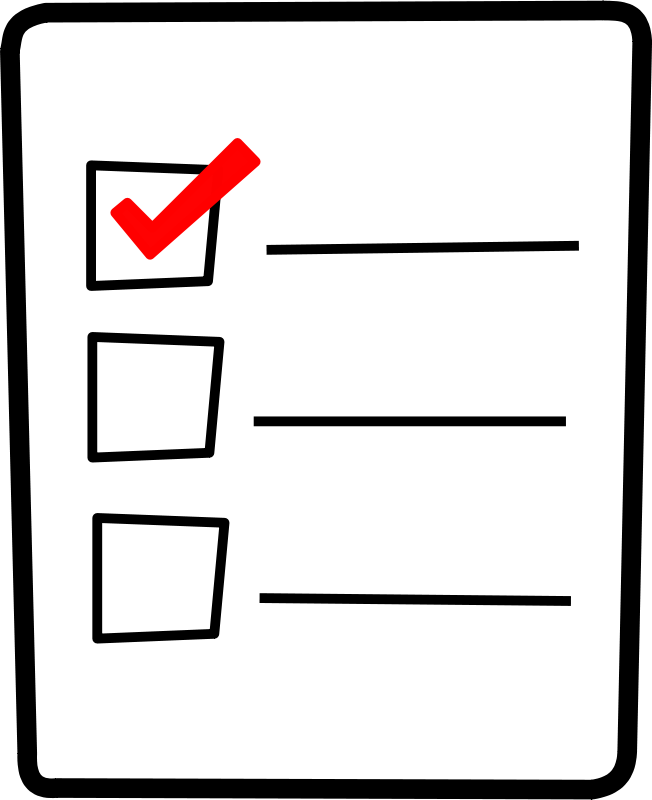
\includegraphics[width=2cm]{checkup.png}
	\end{wrapfigure}%
}

\RequirePackage{longtable}
\renewcommand{\arraystretch}{1.3}

\newcommand{\smileys}{\Large\usym{1F604}\xspace\usym{1F642}\xspace\usym{1F610}\xspace\usym{1F641}}

\newenvironment{checkup}{\begin{longtable}{|p{8cm}|c|p{5cm}|} \hline
		\rowcolor{black!20}
		\rmfamily\textbf{Ich kann ...}
		&
		& \rmfamily\textbf{Informationen \&\newline Aufgaben} \\ \hline\hline\endhead}{\end{longtable}}

\def\ichkann#1#2{#1 & \smileys & %
	\bgroup\def\arraystretch{1}\begin{tabular}{l}
		#2
	\end{tabular}\egroup \\ \hline}

% https://tex.stackexchange.com/questions/4386/defining-starred-versions-of-commands-macro
% und
% https://tex.stackexchange.com/questions/376375/using-ifstar-to-define-a-star-variant
\def\ichkannmulti{\@ifstar\@ichkannmulti\@@ichkannmulti}
\def\@ichkannmulti#1#2#3{#2 & \smileys & \multirow{#1}{*}{#3} \\ \hline}
\def\@@ichkannmulti#1{#1 & \smileys & \\ \cline{1-2}}

\newcommand{\teiler}[1]{\multicolumn{3}{||l||}{\color{gray}\sffamily\bfseries #1} \\ \hline}

\newcommand{\af}[1]{Afg.#1}
\newcommand{\bu}[2]{Buch S.#1\ifthenelse{\equal{#2}{}}{}{, \af{#2}}}
\newcommand{\ah}[2]{AH S.#1\ifthenelse{\equal{#2}{}}{}{, \af{#2}}}